\documentclass[margin=5mm, tikz]{standalone}
\usepackage[utf8x]{inputenc}
\usepackage{tikz}
\usepackage{siunitx}
\usepackage{physics}
\begin{document}
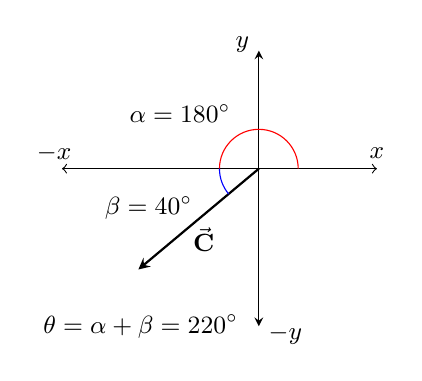
\begin{tikzpicture}
    
    \draw [-stealth, <->] (-2.5, 0) -- (1.5, 0) node [above, pos=1] {\small{$x$}};
    \draw [-stealth] (0, 0) -- (0, 1.5) node [left, pos=1.05] {\small{$y$}};
    \draw [-stealth] (0, 0) -- (0, -2) node [right, pos=1.05] {\small{$-y$}};
    \node at (-2.6, 0.2) {\small{$-x$}};

    \draw [-stealth, thick] (0, 0) -- (-1.53, -1.28);
    \node at (-0.7, -0.9) {\small{$\va{C}$}};
    % \node at (-1.7, 1.4)  {\small{$\va{d} = \SI[per-mode=symbol]{10}{\meter\per\second}$}};
    \draw [color=red] (0.5, 0) arc(0:180:0.5);
    \node at (-1, 0.7) {\small{$\alpha = \ang{180}$}};
    \draw [color=blue] (-0.5, 0) arc(180:220:0.5);
    \node at (-1.4, -0.5) {\small{$\beta = \ang{40}$}};

    \node at (-1.5, -2) {\small{$\theta = \alpha + \beta = \ang{220}$}};
    

    % \draw [color=red] (-0.5, 0) arc(180:150:0.5);
    % \node at (-1.3, 0.25) [color=red] {\small{$\varphi = \ang{30}$}};

    % \node at (-1.5, 1.6) {\small{$\theta + \varphi = \ang{180}$}}
    % \draw [-stealth, thick] (2, 0) -- (2, 2) node [right, midway] {$A_{y}$}; 
    % \draw [-stealth, thick] (0, 0) -- (2, 0) node [below, midway] {$A_{x}$};

    % \draw (1.6, 0) -- (1.6, 0.2) -- (2, 0.2);
    
\end{tikzpicture}
\end{document}